\documentclass{article}
\usepackage{fullpage,amsmath,amsthm,graphicx,enumitem}
\usepackage{multicol}
\usepackage{booktabs}
\usepackage{blkarray}

\usepackage{tikz}

\theoremstyle{definition}
\newtheorem{thm}{Theorem}
\newtheorem{question}[thm]{Question}
\newenvironment{solution}{\noindent\textit{Solution:}}{}

\title{ASEN 5519-002 Decision Making under Uncertainty\\
       Quiz 3: Bayesian Networks and Games}

\date{\small Show all work and justify and box answers.\\
You may consult any source, but you may NOT communicate with any person except the instructor.
}

\begin{document}
\maketitle

\begin{question} (40 pts)
    Consider the following Bayesian network structure:

    \begin{center}
    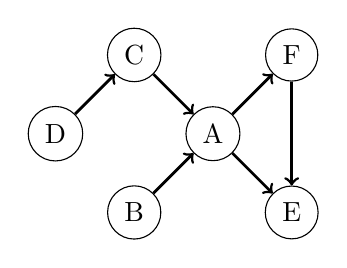
\begin{tikzpicture}
        \node[shape=circle,draw=black] (D) at (0,0) {D};
        \node[shape=circle,draw=black] (A) at (2,0) {A};
        \node[shape=circle,draw=black] (C) at (1,1) {C};
        \node[shape=circle,draw=black] (F) at (3,1) {F};
        \node[shape=circle,draw=black] (E) at (3,-1) {E};
        \node[shape=circle,draw=black] (B) at (1,-1) {B};
        \path [->,line width=1pt] (D) edge node[left]{}(C);
        \path [->,line width=1pt] (C) edge node[left]{}(A);
        \path [->,line width=1pt] (B) edge node[left]{}(A);
        \path [->,line width=1pt] (A) edge node[left]{}(E);
        \path [->,line width=1pt] (A) edge node[left]{}(F);
        \path [->,line width=1pt] (F) edge node[left]{}(E);
    \end{tikzpicture}
    \end{center}

    \begin{enumerate}[label=\alph*)]
        \item True or Inconclusive given structure: $E\perp C \mid F$? Justify your answer.
        \item True or Inconclusive given structure: $E\perp C \mid A$? Justify your answer.
        \item Suppose that all random variables in the network are binary. Given the following conditional distributions and evidence values, infer the probability of $C=1$.
            \begin{itemize}
                \item $P(C=1 \mid D=1) = 0.8$
                \item $P(A=1\mid C=1) = 0.7$
                \item $P(A=1\mid C=0) = 0.4$
                \item Evidence: $D=1$, $A=0$
            \end{itemize}
        \item Suppose that $P(E=0 \mid C=0, A=1, F=1) = 0.4$. What is $P(E=1 \mid C=1, A=1, F=1)$? Justify your answer.
    \end{enumerate}
\end{question}
\clearpage
\begin{question} (30 pts)
    Answer the following questions about simple games:
    \begin{enumerate}[label=\alph*)]
        \item Does the following game have a Nash equilibrium? Justify your answer.
            \begin{center}
                \begin{tabular}{cc}
                & Player 2\\
                    Player 1 & 
            \begin{tabular}{c|c|c|}
            & a & b \\ \hline
            a & 1,2 & 2,1 \\ \hline
            b & 2,1 & 1,2 \\ \hline
            \end{tabular}
                \end{tabular}
            \end{center}
        \item Consider the following incomplete game matrix:
            \begin{center}
                \begin{tabular}{cc}
                & Player 2\\
                    Player 1 & 
            \begin{tabular}{c|c|c|}
            & a & b \\ \hline
            a & 10,10 & 3,5 \\ \hline
            b & 5,3 & $x$,$y$ \\ \hline
            \end{tabular}
                \end{tabular}
            \end{center}
            Choose $x$ and $y$ so that the game has two pure Nash equilibria.
        \item In the incomplete game matrix above, choose $x$ and $y$ so that the game has a single dominant strategy equilibrium.
    \end{enumerate}
\end{question}

\begin{question} (30 pts)
    Consider a turn taking game where Player 1 (the maximizing player) chooses a number between 1 and 3 (i.e. 1, 2, or 3) then, after seeing Player 1's number, Player 2 also chooses a number between 1 and 3. If \emph{both} the sum of the two numbers \emph{and} the product of the two numbers are even, Player 2 wins, otherwise, Player 1 wins.
    \begin{enumerate}[label=\alph*)]
        \item Draw a minimax tree depicting this game labeled with payoffs.
        \item Use minimax backup to calculate the values at each node and indicate them on the tree.
        \item Which player has the advantage?
        \item What number should Player 1 choose?
    \end{enumerate}
\end{question}

\end{document}
